\documentclass{ubicomp2011}
\usepackage{times}
\usepackage{url}
\usepackage{graphics}
\usepackage{color}
\usepackage[pdftex]{hyperref}
\hypersetup{%
pdftitle={Info@ITU}, pdfauthor={Egil Hansen, Jonas Rune Jensen}, pdfkeywords={ITU, BLIP, Android, Mandatory Assignment}, bookmarksnumbered, pdfstartview={FitH}, colorlinks,
citecolor=black, filecolor=black, linkcolor=black, urlcolor=black,
breaklinks=true, }
\newcommand{\comment}[1]{}
\definecolor{Orange}{rgb}{1,0.5,0}
\newcommand{\todo}[1]{\textsf{\textbf{\textcolor{Orange}{[[#1]]}}}}

%\pagenumbering{arabic}  % Arabic page numbers for submission.  Remove this line to eliminate page numbers for the camera ready copy

\begin{document}
% to make various LaTeX processors do the right thing with page size
\special{papersize=8.5in,11in}
\setlength{\paperheight}{11in}
\setlength{\paperwidth}{8.5in}
\setlength{\pdfpageheight}{\paperheight}
\setlength{\pdfpagewidth}{\paperwidth}

% use this command to override the default ACM copyright statement
% (e.g. for preprints). Remove for camera ready copy.
\toappear{}



\title{Info@ITU}
\numberofauthors{2}
\author{
  \alignauthor Egil Hansen\\
    \affaddr{IT University of Copenhagen}\\
    \email{ekri@itu.dk}
 \alignauthor Jonas Rune Jensen\\
    \affaddr{IT University of Copenhagen}\\
    \email{jrur@itu.dk}}

\maketitle

\section{Introduction}

Our Info@ITU system is build up of three main components, a monitor, a cloud based proxy, and a Android app. The monitor tracks the user while inside ITU and displays information to the user when the user is close to a display, the app keeps track of when the user leaves or enters ITU, and the proxy enables the app to communicate with the monitor. The deployment diagram in figure \ref{fig:deployment-diagram} illustrates this.

The Info@ITU system only really relies on location as context, but it is easy to imaging a few extensions that would increse the value and usability of the system.

Location could be enhanced with accelorametor and a compas sensor to the Android app, that would allow the Android app to determine if the user has been sitting still for a while,
e.g. at a session. A combination of an accelorametor and a compas could help determine if a user is standing still and actually facing a display to see his information, or is just moving past it or not looking at it.

Another enhancement would be to also consider if other users is standing in front of a display, which may be able to solve privacy concerns, i.e. by filtering away private information from the display if the user is not alone in front if it.

Considering the fact that the main scenario is ITU hosting a Ubicomp conference, adding time and date to the context is a given. It could, for example, help automatically show upcoming sessions.og

\begin{figure}[t]
\begin{center}
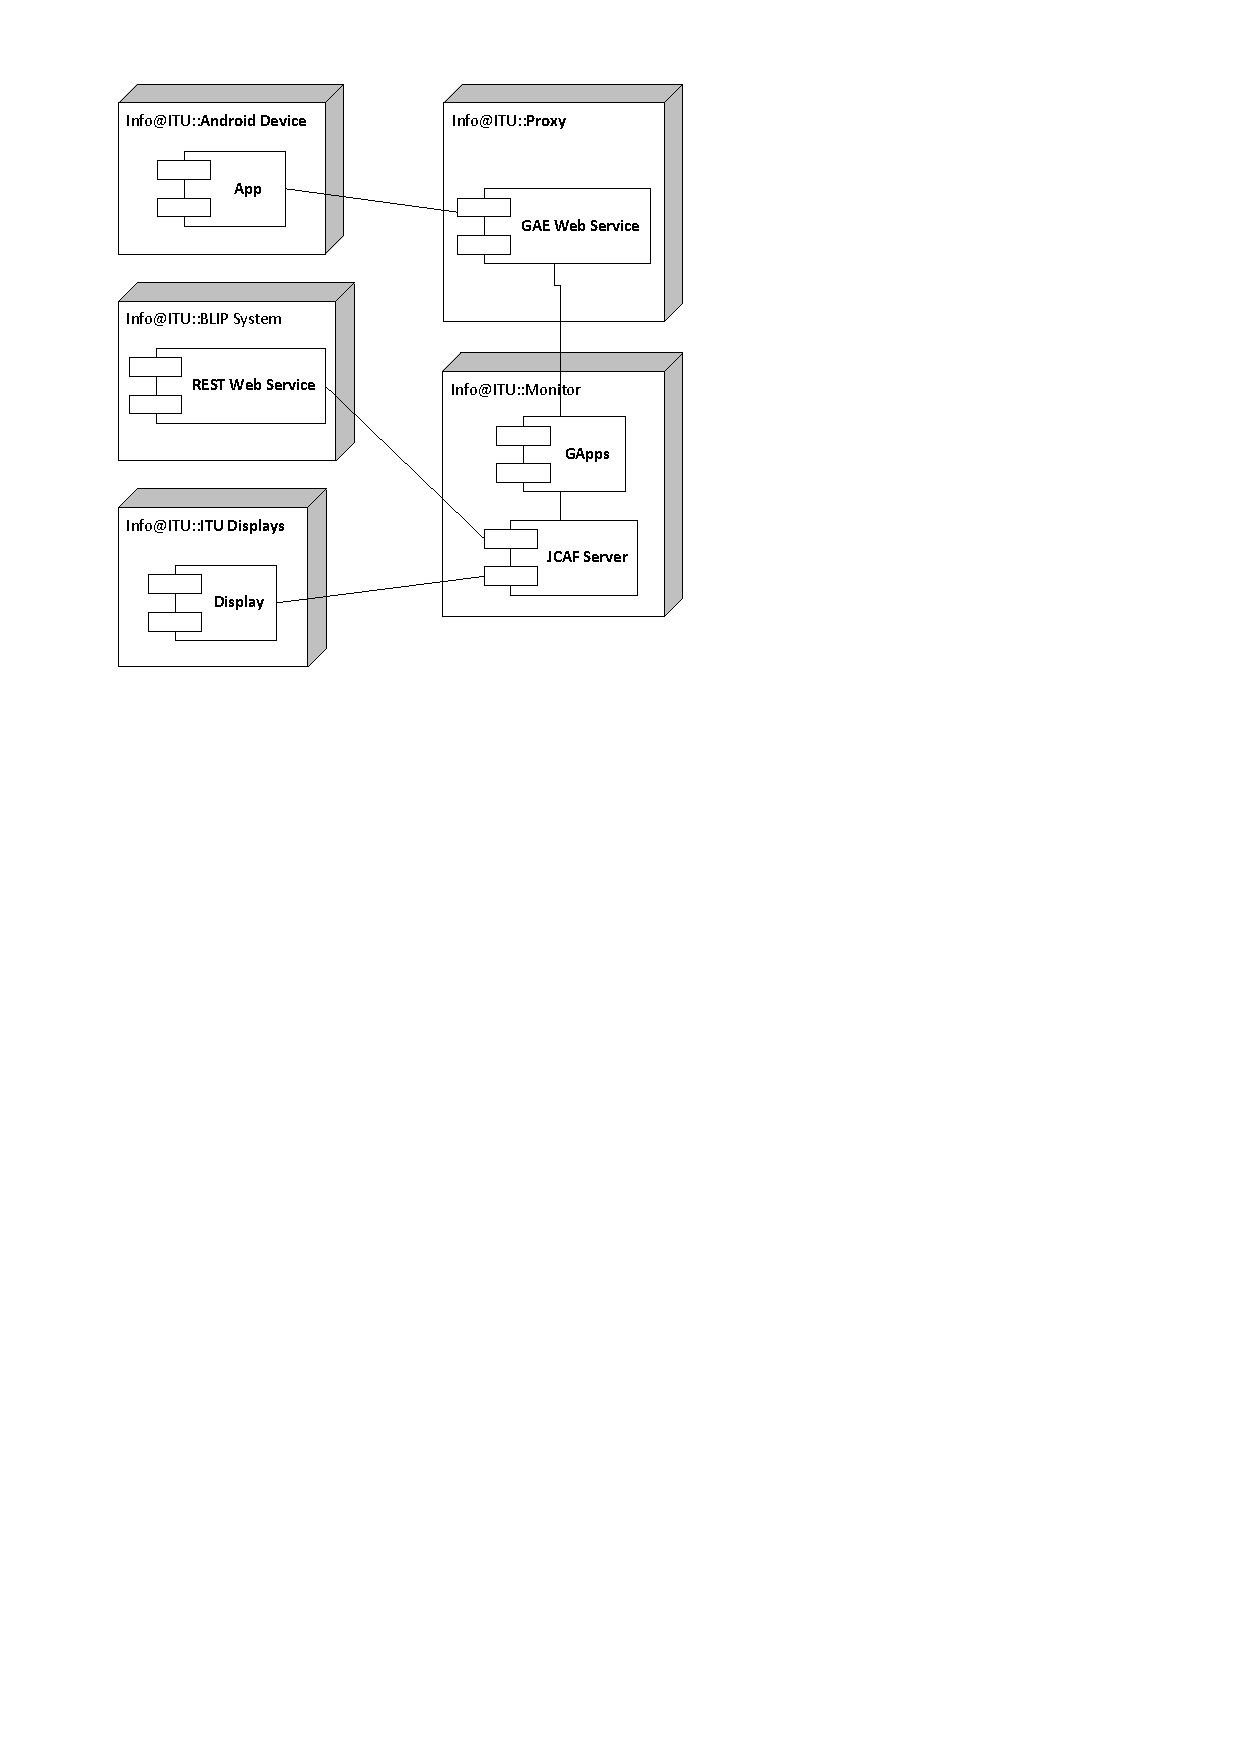
\includegraphics[width=0.90\columnwidth]{deployment-diagram.pdf}
\end{center}
\caption{Deployment diagram for our Info@ITU system.}
\label{fig:deployment-diagram}
\end{figure}
\subsection{Context-Aware Applications}

\section{Info@ITU Monitor}

To be able to track our users at ITU, we are using a combination of JCAF and the BLIP system where JCAF has all the information about the user and displays the relevant information to the designated monitor, and BLIP is used to keep watch of were the users is at ITU.
The first thing that we designed for our JCAF system was a jar called dk.itu.info.jar, which contains all the objects that is going to be used in our system. As JCAF is a RMI system we need to have the same type of objects both at the server and in the different components as monitors and listeners.

We have two entities, a Visitor and a Room. These contains information about the id and name of the person, and id, floor, sector and room of the room. For our person the id is going to be the mac address of the bluetooth device we are tracking, which could be something like “E4B0219CE1AD”, and for the room it is the string that represents a Blip node like “itu.zone2.zone2c”.
We have used three different types of actuators to represent the different states that a user can be in, these are Left, Arrived and Located. Arrived is used when a user is arriving at a location, Located is used when we know that a user is Arrived and is still at the same location, and last Left is when a user has left ITU or is sign out and a display needs to be empty.

In order to know if the user is at ITU

-areas:
Gapps
- registrere når at bruger forsvinder fra list og sætter vedkommende som left
Blipmonitor
- kunne tælle hvis en bruger er null så er man væk
- blip er kun tilgængeligt i små områder
AreaListener
\section{Info@ITU Proxy}

The proxy is available at http://info-at-itu-proxy.appspot.com and provides the following service methods for the monitor and mobile devices:

\begin{itemize}
\item \texttt{entering?<BT MAC address>\&<Username>}\\
This method is used by the phone to tell the system that the phone is moving into ITU and to start tracking the it.
\item \texttt{leaving?<BT MAC address>}\\
This method is used by the phone to tell the system that the phone has left ITU and to stop tracking it.
\item \texttt{ping?<BT MAC address>}\\
This method should be used every XX minutes, after the phone has entered into ITU, to indicate to the system that the phone is still turned on and inside ITU.
\item \texttt{getallclients}\\
This method returns a JSON formatted aray of all clients that have been `checked in’ with the proxy.
\end{itemize}

The reason why we added the \texttt{ping} method is to handle the common scenario where the phone is out of range of ITU's BLIP sensors for a longe time, i.e. when the owner is in a meeting room or lecture hall, or if the owner has turned of his phone or the phone has simply run out of power. If the proxy stops receiving pings from the phone, we assume that the phone should no longer be tracked and can save resources on the monitor.
\subsection{Future Work}

A related feature to the \texttt{ping} method, which is not yet implemented, is a scheduled clean-up job, that searches through the list of `checked in' phones on the proxy and removes those who have not `pinged in' for 20 minutes.

Push notificaitons from the proxy to the monitor would also be natural extension, since it would lower the resources required and allow the monitor to be notified almost instantly when a new phone `checks in'. In the current solution, the monitor pulls from the server every 15 seconds to see if there are any new phones or phones that have left.
\section{Info@ITU App}

For our Info@ITU App we considered the problems with identification (who is actually using the Android device), battery life, and volatile state.
\paragraph{Identification}

This is an issue even if mobile phones are often very personal, since they could be shared between people, or more likely, a person could have a private profile and a public profile. So to identify the user of the phone, we ask the user to select one of his Google accounts when signing in to Info@ITU from his device. This also enable the scenario where a user switches between devices or is signed in with multiple devices, since we identify him and his devices by his Google ID, not by an MAC address.
\paragraph{Battery life}

This can quickly become an issue when both WiFi, GPS and Bluetooth radios are turned on. So we try to be as effective as possible, only turning on Bluetooth when the device is actually inside ITU.
\paragraph{Volatile state}

The volatile state of mobile devices must also be considered -- the user can choose to turn it of, the device can run out of battery, the user can turn of Bluetooth or GPS, other applications can turn of Bluetooth or GPS, all things we need to consider when building an app like this that relies on these.

\begin{figure}[t]
\begin{center}
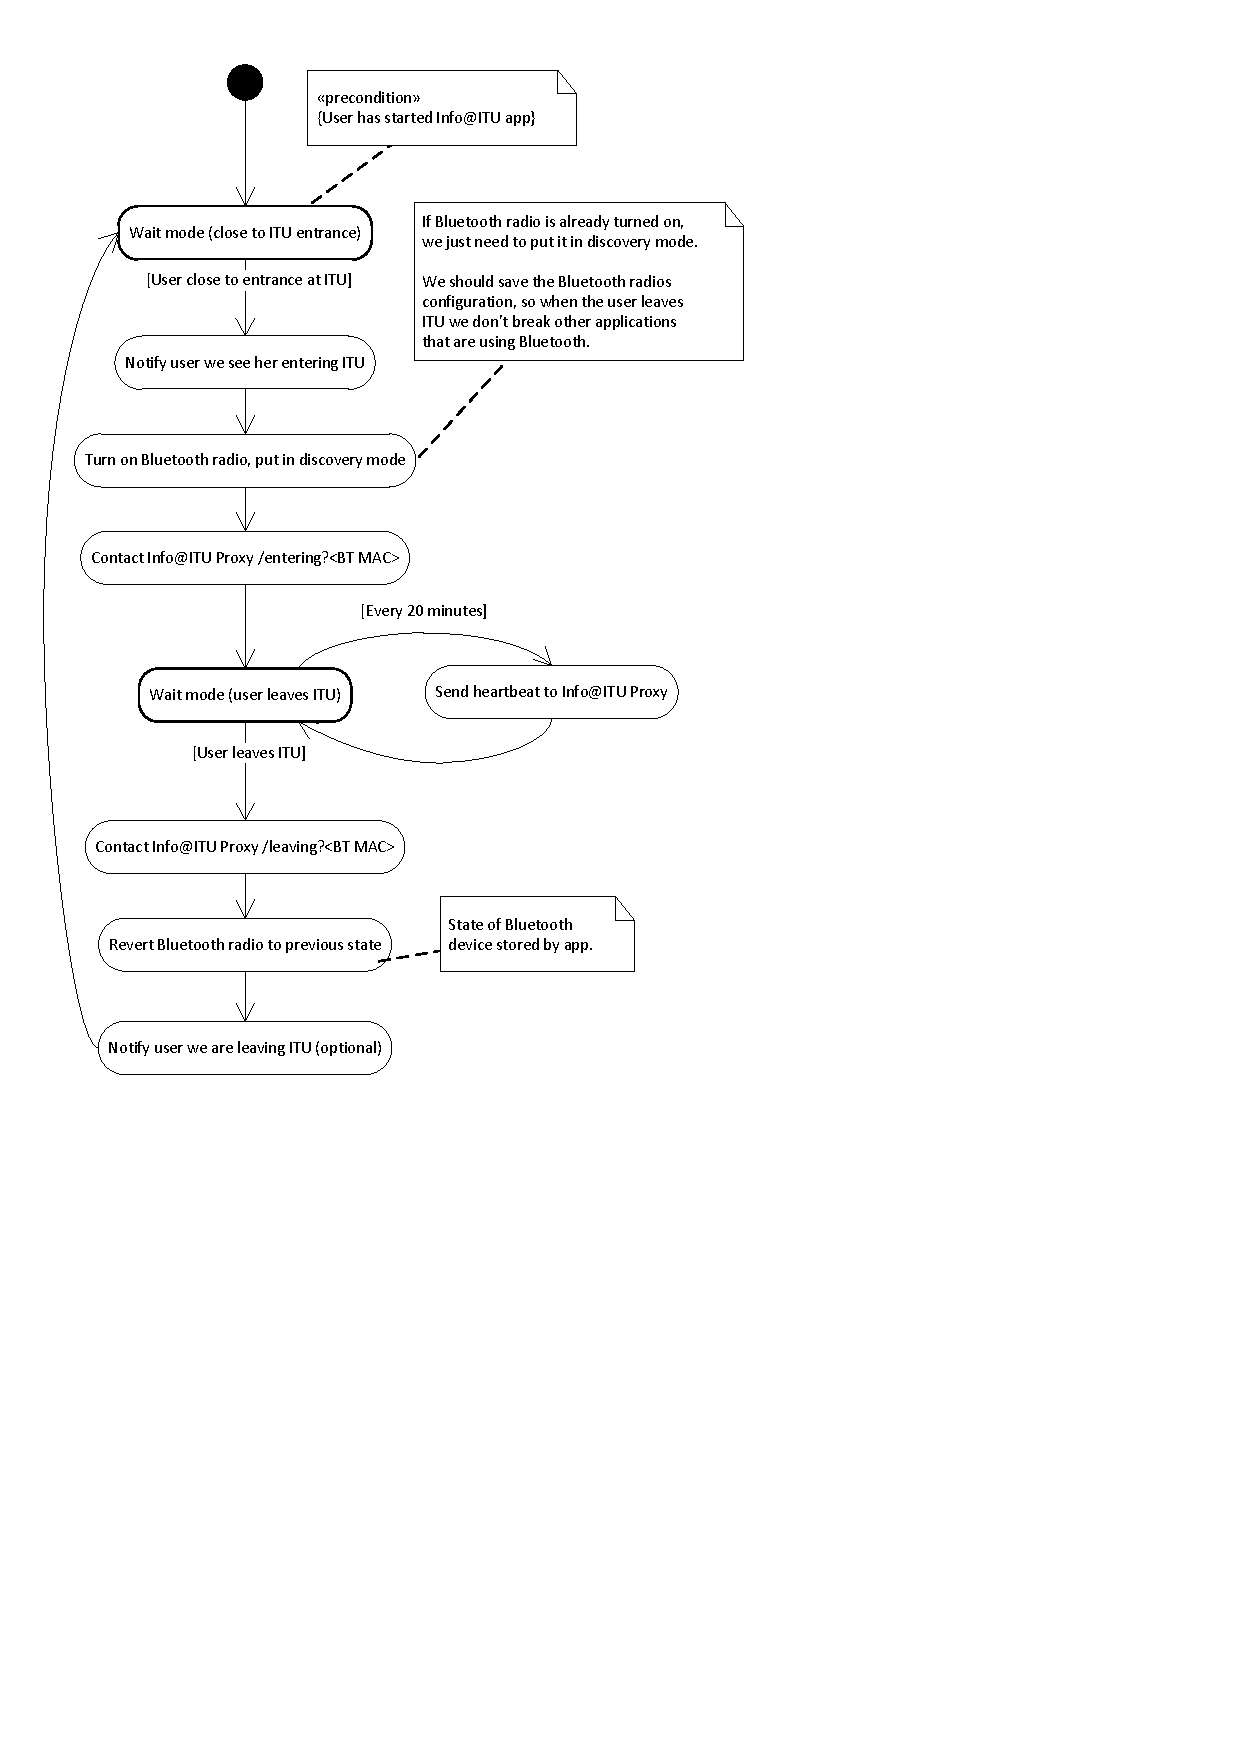
\includegraphics[width=0.90\columnwidth]{android-app-activity-diagram.pdf}
\end{center}
\caption{Activity diagram for the Info@ITU App.}
\label{fig:android-app-activity-diagram}
\end{figure}

The workflow of our App is illustrated in figure \ref{fig:android-app-activity-diagram}. Before we enter into the initial waiting state in the figure, the user is asked  to sign in to our application with a Google ID of his choice.

\end{document}